\chapter{Processo de Desenvolvimento}
\label{cha:rivers_implementation}

Rivers surgiu da necessidade de se implementar soluções simples porém eficientes para o processamento de grandes volumes de dados. Na empresa Bearch Inc esse processo é recorrente e pela falta de uma solução nativa no contexto da linguagem de programação Go utilizada amplamente nos projetos internos da empresa, desenvolvedores acabavam por implementar lógicas de processamento redundantes que se repetiam ao longo do desenvolvimento de vários projetos. Devido aos custos deste retrabalho e aos padrões encontrados no processo de desenvolvimento de vários projetos, foi proposto uma solução para ajudar a reduzir a quantidade de código necessário para se implementar essas rotinas de processamento assim como possibilitar o reuso de lógicas existentes de soluções anteriores.

Este capítulo discute brevemente o processo de desenvolvimento empregado assim como as práticas utilizadas para guiar a evolução da solução minimizando a quantidade de retrabalho necessário ao longo das iterações.

\section{Coleta de Requisitos e Roadmap}
\label{sec:requirements}

Requisitos foram levantados afim de se ter um conjunto mínimo de funcionalidades que pudesse formar o MVP inicial para que se iniciasse o desenvolvimento. A tabela \ref{mvp:requirements} lista as features consideranas no Roadmap de Rivers, algumas delas selecionadas para compor o MVP e outras implementadas somente na versão seguinte. As features marcadas para compor o MVP foram selecionadas com o intuito de se ter o mínimo de funcionalidades disponíveis para se implementar um pipeline de processamento de streams que possa ser utilizado em diferentes contextos já identificados em projetos anteriores da empresa, como por exemplo no processamento de entidades da base de dados assim como no processamento de resultados de chamadas de APIs de outros sistemas.

\begin{table}[h!]
    \centering
    \begin{tabular}{||c c c||} 
        \hline
        Backlog & MVP & V2.0 \\ [0.5ex] 
        \hline\hline
        Contexto Global & X & \\ 
        \hline
        Producer Interface & X & \\ 
        \hline
        Producers Especializados (List, Socket, File...) & & X \\ 
        \hline
        Transformer Interface & X & \\ 
        \hline
        Transformers Especializados (Map, Each, Filter...) & & X \\ 
        \hline
        Consumer Interface & X & \\
        \hline
        Consumers Especializados (Count, Reduce...) & & X \\
        \hline
        Dispatchers & & X \\
        \hline
        Combiners & & X \\
        \hline
        Panic Recovering & X & \\
        \hline
        Failure Retries & & X \\
        \hline
        Suporte a Paralelização & & X \\
        \hline
        Pipelines Distribuídos & & X \\ [1ex]
        \hline
    \end{tabular}
    \caption{Rivers Roadmap: MVP vs. V2.0}
    \label{mvp:requirements}
\end{table}

Afim de atender as necessidades dos projetos utilizados como casos de uso, foi decidido então que uma solução útil e viável teria que prover pelo menos uma implementação genérica de cada um dos estágios que compõem um pipeline. Um Producer deveria permitir com que diferentes fontes de dados sejam utilizadas no pipeline como geradores de dados como por exemplo base de dados, APIs Restful e arquivos. Uma implementação de Transformer deve permitir que uma lógica específica de processamento possa ser aplicada aos dados sendo transmitidos pelo stream e seu resultado passado ao próximo estágio. Um Consumer por sua vez deve permitir que dados possam ser coletados de maneira síncrona ao final do pipeline assim como possíveis erros de execução. Por fim, a implementação inicial deveria prover um mecanismo simples que pudesse detectar falhas em tempo de execução notificando-as aos estágios do pipeline para que os mesmos possam suspender sua execução.  Implementações mais especializadas de cada um destes estágios seriam o foco em versões futuras da API como por exemplo producers especializados em leitura de arquivos, drivers de base de dados específicas, transformers especializados em operações como Map, Reduce, Filter, etc, mecanismos para se executar o pipeline de maneira distribuída em um cluster de máquinas.

O plano de desenvolvimento foi mantido e disponibilizado como GitHub \ref{github} issues apresentado através de um dashboard Kanban \ref{kanban} disponível em Waffle.io \ref{waffle} para facilitar a visualização do progresso mantendo a informação e comunicação centralizada, como mostrado na figura \ref{fig:waffle}. Ao longo do desenvolvimento, cada feature implementada era prontamente testada em casos de uso reais por outros desenvolvedores e feedbacks coletados afim de aprimorar a solução de acordo com as necessidades reais do time.

\begin{figure}[H]
  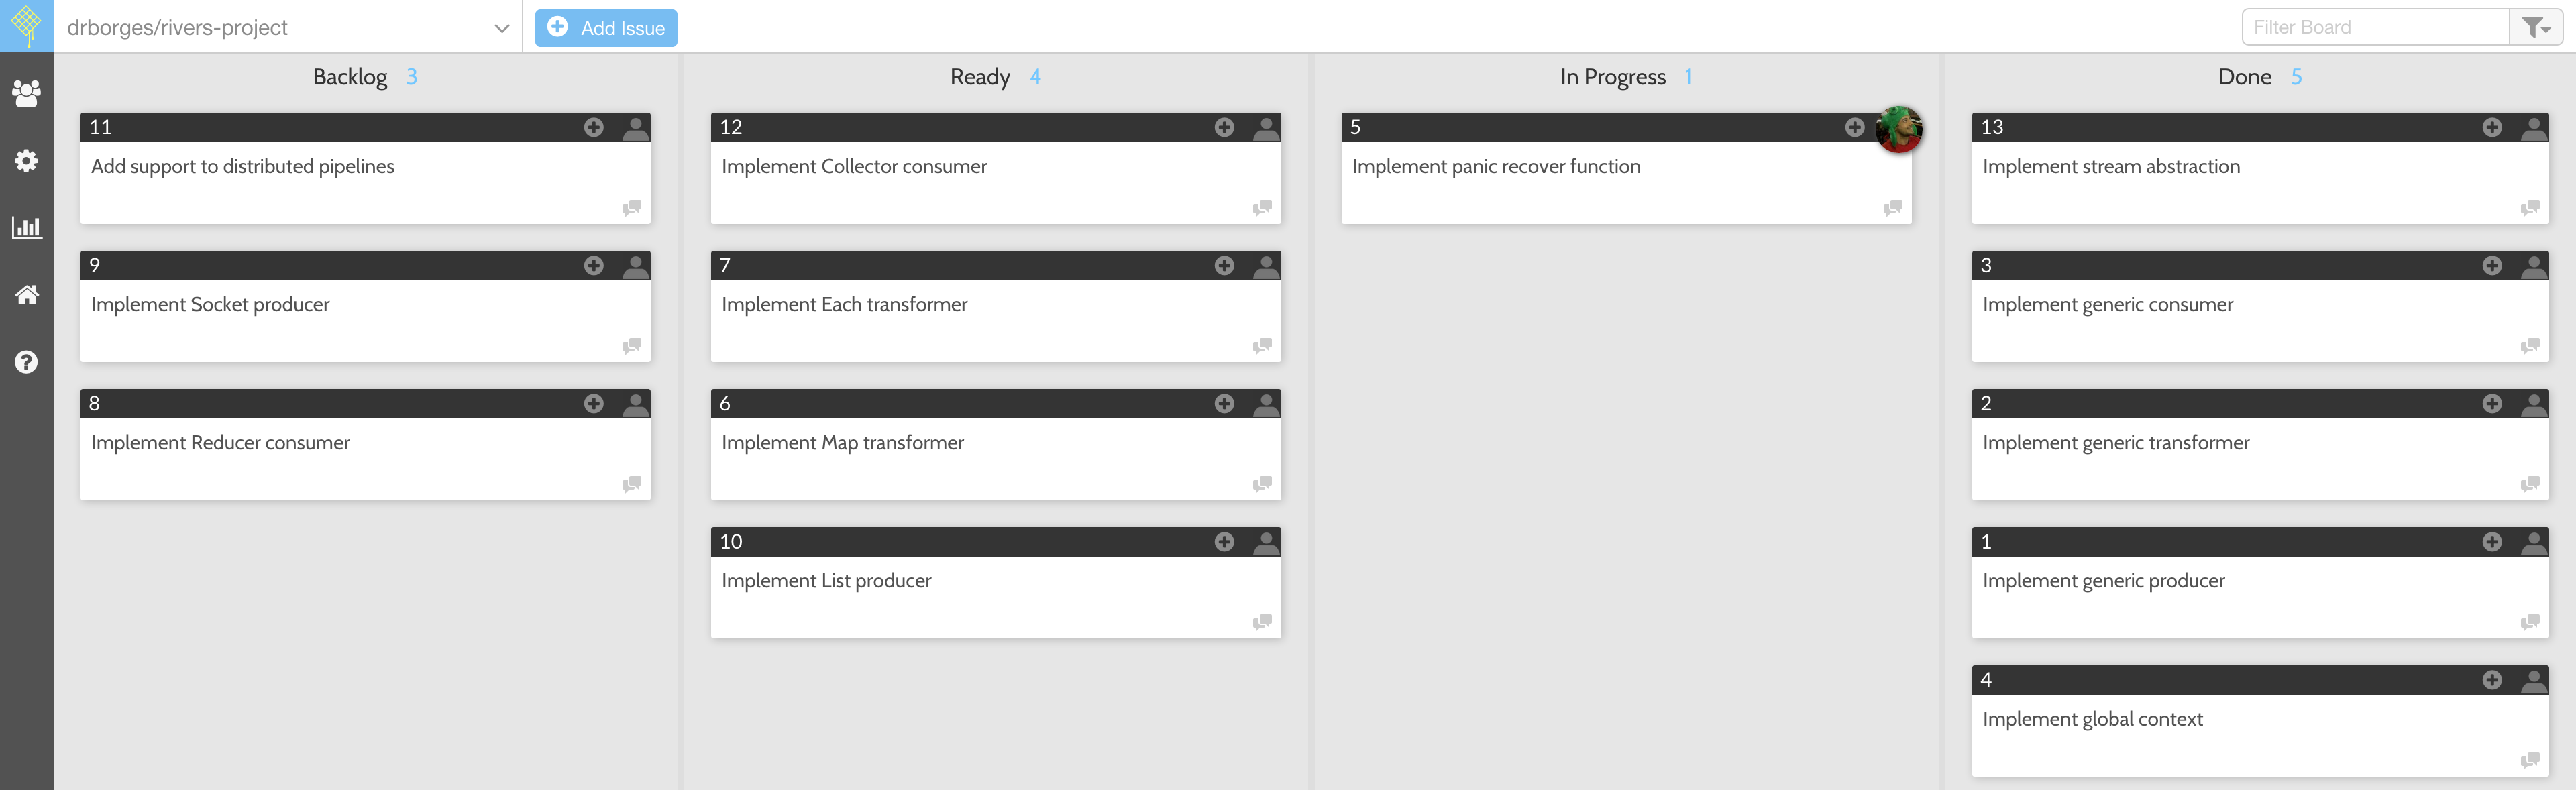
\includegraphics[width=1\textwidth]{waffle}
  \centering
  \caption{Roadmap visualizado em um dashboard Waffle.}
  \label{fig:waffle}
\end{figure}

\section{Tests \& Benchmarks}
\label{sec:tests_n_benchmarks}

Foi utilizada a técnica Test Driven Development \cite{book:tdd:kent_beck} para toda nova funcionalidade implementada. Escrevendo-se os casos de teste antes mesmo de se ter a funcionalidade ajudou a guiar o design da API gradativamente, uma vez que toda complexidade envolvida na implementação da nova funcionalidade era colocado inicialmente de lado, permitindo o desenvolvedor focar no design da API se colocando como usuário da mesma em um primeiro momento. Através do uso desta técnica, foi possível alcançar uma cobertura de testes razoável criando um conjunto de testes de regressão muito útil na detecção de quebra de funcionalidades já existentes devido a alterações de certas áreas do codebase. Visando tirar o máximo de proveito da técnica, foi utilizado a ferramenta fsnotify \cite{tools:fsnotify} para execução dos testes de regressão sempre que um arquivo no codebase é alterado, disponibilizando um relatório dos resultados de cada teste executado com isso um feedback instantâneo com relação as últimas alterações no codebase. A figura \ref{fig:tdd-cycle} representa o ciclo de desenvolvimento seguido aplicando a técnica TDD.

\begin{figure}[H]
  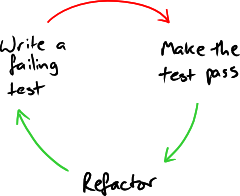
\includegraphics[width=0.4\textwidth]{tdd-cycle}
  \centering
  \caption{Ciclo de desenvolvimento aplicando a técnica TDD.}
  \label{fig:tdd-cycle}
\end{figure}

Alguns benchmarks foram implementados para medir a eficiência de um pipeline segundo a solução proposta em comparação com soluções utilizada previamente em outros projetos. A tabela a seguir mostra os resultados medidos entre duas versões de um Job que processa 1000 entidades datastore por vez aonde o processamento leva em média 1 seg por entidade. Em uma versão foi implementado um pipeline Rivers com paralelização ativada afim de tirar o máximo de proveito do hardware utilizado. A outra implementação segue uma solução sequencial utilizada anteriormente em outros projetos.

\begin{table}[h!]
    \centering
    \begin{tabular}{||c c c||} 
        \hline
        Jobs & Número de Goroutines & Tempo Médio de Execução (seg) \\ [0.5ex] 
        \hline\hline
        Pipeline Rivers & 1000 & 1.16 \\ 
        \hline
        Solução Sequencial & 1 & >1000 \\ [1ex]
        \hline
    \end{tabular}
    \caption{Comparação entre Jobs sequencial e Rivers paralelizado}
    \label{benchmarks:sequential_vs_parallel}
\end{table}